%===================================== CHAP 8 =================================

\chapter{Computational Study}


In this chapter, a computational study based on the solution approach outlined in Chapter 5 is presented. First, in Section \ref{sec:exact}, the optimal solution with perfect information is presented. Secondly, in Section \ref{sec:inexact}, the performance of each of different solution approaches are presented. 

\newpar

The mathematical model is written in the algebraic modelling language Mosel and implemented in FICO\textsuperscript {\textregistered} Xpress Optimization Suite 8.3, using a HP EliteDesk 800 G3 DM 65W computer with Intel\textsuperscript{\textregistered} Core\textsuperscript{\texttrademark} i7-7700 3.6 GHz processor and 32 GB RAM. The operating system in use is Windows 10 Education 64-bit. The input data to the mathematical model is structured and pre-processed in the statistical programming language R. Further, the results obtained from the mathematical model include decisions on selected squad, starting line-up, substitution priority, number of illegal transfers, captain, vice-captain and whether a gamechip is used in a gameweek. These are written to CSV files, which are exported back to R to calculate points the team achieved. In the end, these are further exported to Microsoft Excel to make the data more presentable in form of tables and plots. 

\section{Solution with realized points}\label{sec:exact}
This section is divided in three parts. 
First, the initialization of sets and parameters is presented. Following is a discussion of the problem size and operations research metrics such as optimality gap, bound, computational time and etc. Secondly, the solution is more thoroughly examined to discuss whether the decisions made are sensible or not. Lastly, the solution is compared against the best performing human managers. 



\subsection{Initialization of parameters}    
%DEL1 

Following in table \ref{tab:initializations_of_sets} and \ref{tab:initialization_of_parameters} are the initialization of parameters and sets used when the mathematical model with realized points is solved. 

\begin{table}[H]
\centering
\caption{Initialization of sets.}
\begin{tabular}{@{}lll@{}}
\toprule
Set           &   &                                                               \\ \midrule
$\mathcal{T}$ & - & 35 gameweeks,                                             \\
$\mathcal{P}$ & - & 625 players,                                               \\
$\mathcal{C}$ & - & 20 teams,                                                 \\
$\mathcal{L}$ & - & \{1,2,3\}, where 1 is first priority, \\
$\mathcal{T}_{FH}$ & - & Gameweek 1 to 21 is in the first half of the season,\\
$\mathcal{T}_{SH}$ & - & Gameweek 22 to 35 is in the second half of the season.\\
\bottomrule
\end{tabular}
\label{tab:initializations_of_sets}
\end{table}

\begin{table}[H] 
\tabcolsep=0.11cm
\centering
\caption{Initialization of parameters.}
\begin{tabular}{@{}lll@{}}
\toprule
Parameters                       &   &                                                                                                \\ \midrule
$\mathlarger{\rho_{pt}}$ & - & Realized points for a player $p$ in a gameweek $t$. \\
$\epsilon$                       & - & Set to 0.1.                                                                     \\
$\kappa_{1}, \kappa_{2}, \kappa_{3} $                     & - & Set to 0.01, 0.001 and 0.0001 respectively.                                               \\
$C_{pt}^{B}$                     & - & Buy price collected from FPL homepage.  \\ 
$R$                              & - & 4 points deducted if number of free transfers is exceeded.       \\
$M^{K}$                          & - &  2 goalkeepers required in the selected squad.                                      \\
$M^{D}$                          & - &  5 defenders required in the selected squad.                         \\
$M^{M}$                          & - & 5 midfielders required in the selected squad.                                     \\
$M^{F}$                          & - & 3 forwards required in the selected squad.                                    \\
$M^{C}$                          & - & 3 players allowed to have from the same club.                                \\
$E$                              & - & 11 players required in the starting line-up.                              \\
$E^{K}$                          & - & 1 goalkeepers required in the starting line-up.                                       \\
$E^{D}$                          & - & 3 defenders required in the starting line-up.                  \\
$E^{M}$                          & - & 3 midfielders required in the starting line-up.                                 \\
$E^{F}$                          & - & 1 forward required in the starting line-up.                     \\
$B^{S}$                          & - & 100 million as starting budget.                                                                              \\
$\beta$                          & - & Set to 1.                                                                                  \\          
$\bar{\alpha}$                   & - & Set to 14.                                                                      \\

$\phi$                         & - & 3 players are substitutes.                                                         \\
$\phi^{K}$                   & - & 1 keeper among the substitutes.                                                          \\
$\overline{Q}$                   & - & 2 free transfers possible to accumulate over gameweeks.                                              \\
$\underline{Q}$                  & - & 1 free transfer given every gameweek.                                      \\ \bottomrule
\end{tabular}
\label{tab:initialization_of_parameters}
\end{table}

 
A season in FPL consists of 38 gameweeks, however because of restriction on time, an early decision is made to solve the model for the first 35 gameweeks. The season is divided in two halves, where the first half is from gameweek 1 to 21 and the second part is from gameweek 22 to 35. There are a big number of players in the FPL database, where large part of them have featured in a match while there are some who have not. After removing the players who have not featured in a match, the set resulted in 625 players. 

\newpar

All the parameters specifically stated in the rules of FPL are set accordingly. These include number of points deducted if number of free transfers are surpassed, number of players in different position in both selected squad and starting line-up, maximum players from same club, total of starting budget and the restrictions on free transfers. The parameter in the objective function for vice-captain are set to 0.1, while for the substitution priority, $\kappa_{1}, \kappa_{2}, \kappa_{3}$ these are set to 0.01, 0.001 and 0.0001, respectively. To tighten the formulation as much as possible, the parameters $\beta$ and $\alpha$ are set so to the smallest, but sufficiently high value. $\beta$ is used in constraints \eqref{eq:subst} and \eqref{eq:free_hit_subst} in Chapter \ref{chapter_model_formulation} which concern the substitution priority. Considering the variables adopted are binary, setting the value to 1 is optimal. $\alpha$ is used in constraints \eqref{eq:trans_flow_illegal_transfers}, and is set to highest possible value for number of points-deducting transfers. As there is given 1 free transfer each gameweek and the selected squad consists of 15 players, it is not possible to have more than 14 points-deducting transfers. Hence, the parameter $\alpha$ is set accordingly. 

\newpar

The data on each player's value in a gameweek is collected from FPL's homepage \url{www.fantasy.premierleague.com}. 

\subsection{Problem Size}

Table \ref{tab:computational_statistics} display the problem size of FPLDP with input data from season 2017/18. The problem size are given before and after Presolve. This is a function integrated in Xpress Optimizer with few of its objectives are to reduce redundant variables, eliminate redundant constraints and remove linearly dependent constraints, which consequently reduces the complexity of the problem and improve the computing time. As can be seen from the table, the problem size is huge where the number of both constraints and variables are immense. From the table, it can be observed that the Presolve function is successful in eliminating both variables and elements, but the reduction in constraints is not that severe. A reason for this could be that most of the constraints are linearly independent, and that there is a limited present of empty rows in the FPLDP. In addition, a large part of the $x_{pt}$, $x_{pt}^{freehit}$ and $y_{pt}$ are redundant, as many of them are defined despite few of them are used in the starting line-up and selected squad constraints. The fact that Presolve manage to eliminate such a large number of variables, implies that there should have been used more time and effort on reducing redundant variables in the procedure of implementation. That would most likely been effective in reducing solution time. Nonetheless, it can be argued that since the model only has to be solved once, this can to a certain degree be disregarded. 


\begin{table}[H]
\centering
\caption{Computational statistics for the instance with realized points.}
\label{tab:computational_statistics}
\begin{tabular}{@{}llll@{}}
\toprule
                            & Rows(Constraints)    & Columns(Variables) & Elements \\ \midrule
Original Problem Statistics & 172 034 & 254 425  & 1 052 715  \\
Xpress Presolve Statistics  & 170 750 & 206 689  & 891 995   \\ \bottomrule
\end{tabular}
\end{table}


\subsection{Results of running the model with realized points}


\begin{table}[H]
    \centering
    \caption{Results of implementation of exact solution method.}
    \begin{tabular}{c|c|c|c}
        LP Bound & Best solution & Best bound & Gap  \\
         & & & 
    \end{tabular}
\end{table}

\begin{figure}[H]

    \centering
    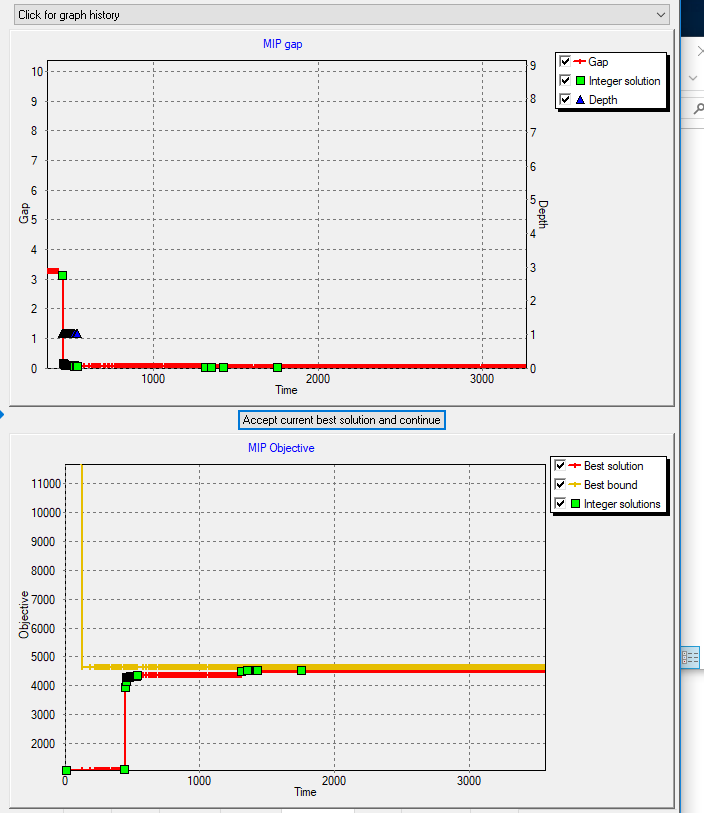
\includegraphics[scale=0.65]{fig/chapter_7/opt_solution_graph.png}
    \caption{Figure of when the solutions are found after how long time.}
    \label{fig:opt_solution_graph}
\end{figure}

\subsection{Performance in Fantasy Premier League}
In the following we provide the results for the model introduced in chapter \ref{chapter_model_formulation} when solved with realized points, i.e. with perfect information. Figure \ref{Figure_Realized_points} gives an overview of how many points the model obtained in each gameweek. The coloured dots represents gameweeks where the gamechips were used. 

\begin{figure}[H]
\label{fig:Realized_points}
    \centering
    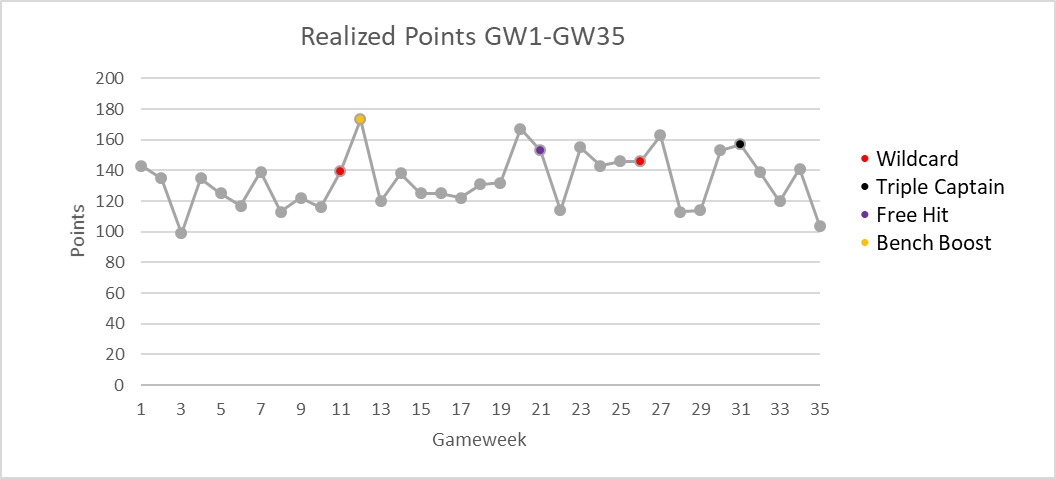
\includegraphics[scale=0.75]{fig/chapter_7/RealizedPoints_colour.png}
    \caption{The graph shows the points per gameweek with perfect information}
\label{Figure_Realized_points}    
\end{figure}

\begin{comment}
We find it necessary to comment on the choices made for selecting when to play the gamechips.
\end{comment}
 As observed, the first wildcard was used one week ahead of the bench boost was played. This is reasonable as it is wisely to ensure that you select 15 players that will earn lots of points when playing the bench boost. Further, the free hit chip was used in gameweek 21, which was a blank gameweek containing only 9 fixtures. It is reasonable to assume that the free hit should either be used ahead of a blank or ahead of a double gameweek in order to ensure that all your selected players are featured at least once for that particular gameweek. Finally, the triple captain chip was used in gameweek 31 which is reasonable as Mohammed Salah scored 4 goals and had 1 assist in this particular gameweek, yielding a score of 29 points. This was the highest score obtained in one gameweek by any Premier League players. As for the second wildcard, there is no obvious reason why it was played in gameweek 26, except the fact that it was optimal for the entire solution. 
\newpar
Figure \ref{Figure_Transfers} shows how many transfers the model made ahead of each gameweek. It is notable that the model performs most transfers when the wildcards and the free hit were played. This makes sense as these chips allows you to perform unlimited free transfers. In general, one can say that the model makes many transfers compared to human managers. However, this is due to the fact that this is an optimal solution. Thus, it selects the players that over-performed in a particular gameweek. Every gameweek there are some players that surprise the FPL managers. For instance, if a defender suddenly scores two goals in a match, the goals themselves yield 12 points. 

\begin{figure}[H]
\label{fig_Transfers}
    \centering
    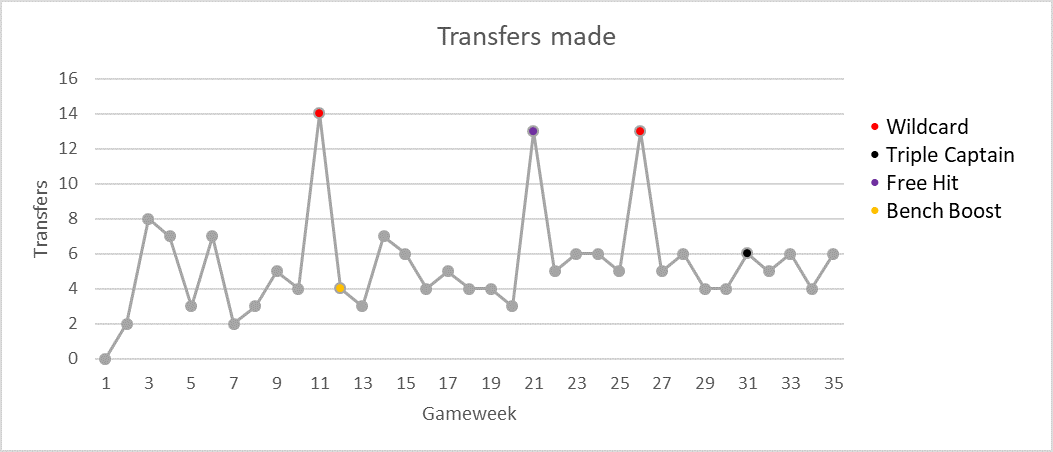
\includegraphics[scale=0.75]{fig/chapter_7/Transfers_colour.png}
    \caption{The graph shows how many transfers the optimal solution makes in every gameweek}
\label{Figure_Transfers}    
\end{figure}

Some readers may find value in comparing the optimal FPL solution to the performance of human managers. Figure \ref{Figure_Comparison} provides a weekly comparison of the weekly average score and the maximum score obtained by human managers to the optimal solution.

\begin{figure}[H]
\label{fig:Comparison}
    \centering
    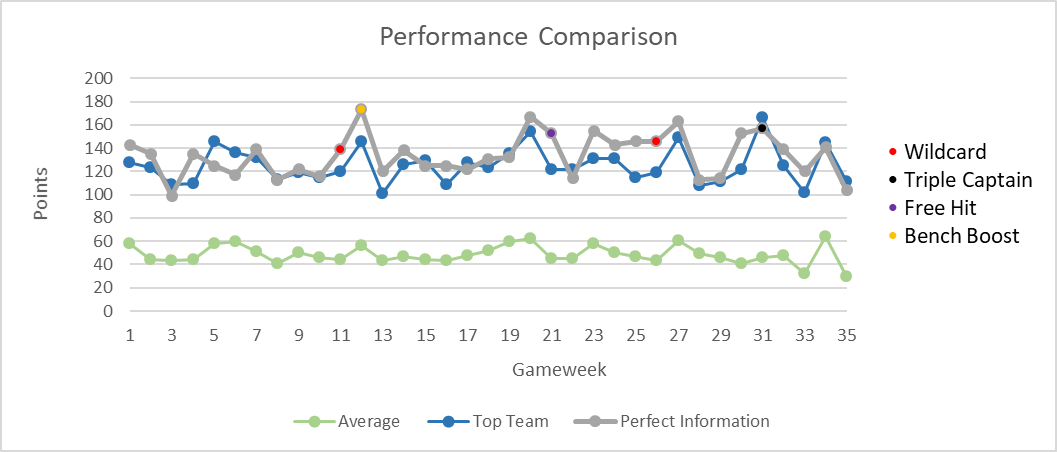
\includegraphics[scale=0.75]{fig/chapter_7/Comparison_colour.png}
    \caption{The graph compares the weekly average and the top performer of each Gameweek to the optimal team with perfect information}
\label{Figure_Comparison}    
\end{figure}

 It is notable that the optimal solution performs well ahead of the weekly average managers, scoring at least twice as many points in every gameweek. Further, it is worth noticing that the optimal overall solution may be beaten by the best manager in individual gameweeks. This is due to the fact that the optimal solution maximizes the points over the entire season, and not only over one particular gameweek. Further, managers that finish top of the gameweek often use a gamechip in order to maximize their weekly score. 
\newpar
There seem to be some positive correlation between the optimal solution and both the weekly top performers as well as the weekly average scores. From table \ref{Figure_Comparison} one can see that the weekly average and the optimal solution have a tendency of moving in the same direction. Hence, when the optimal solution receive a high score, the weekly average have a tendency of doing the same. This might be due to highly selected players performing well in those particular gameweeks. For instance, if a player that has performed well over the entire season receives an abnormal high score during a gameweek, it is anticipated that the weekly average will increase as most managers select this player. Consider Mohamed Salah, who has had an incredible season. At some point he was selected by more than 63\% of the human managers. Thus, when he performs well it is reasonable to assume that both the average and the optimal solution earn numerous points. 
\newpar
As stated in chapter \ref{introduction} it is interesting to compare the optimal solution strategy to that of the manager of leads the overall ranking. Figure \ref{Top_Manager} provides a weekly overview of this comparison.

\begin{figure}[H]
\label{fig:Top_Manager}
    \centering
    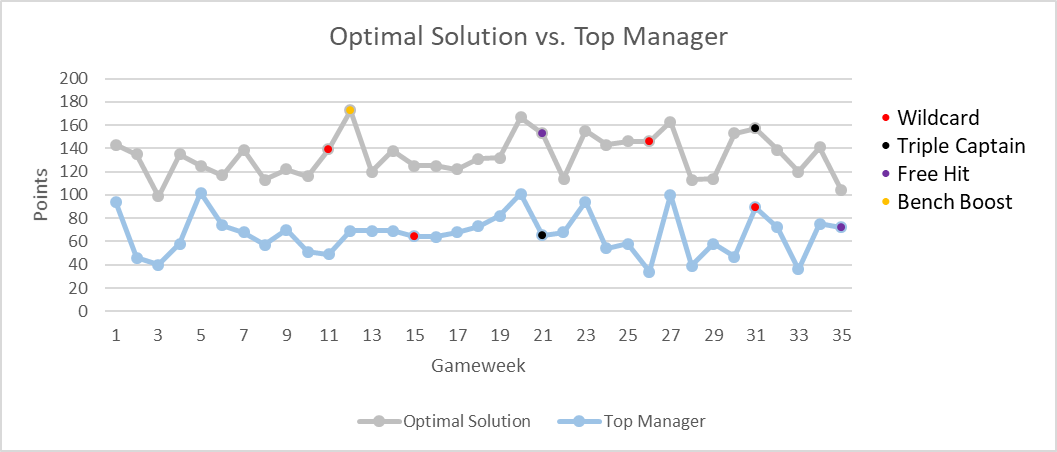
\includegraphics[scale=0.75]{fig/chapter_7/Optimal_vs_Top_colour.png}
    \caption{Comparing optimal solution strategy to top manger}
\label{Top_Manager}    
\end{figure}

As suggested in the introduction, the optimal solution strategy largely outperforms that of the top manager of Fantasy Premier League. In total, it separates 2348 points between the two solutions, more than twice the amount of points gained by the top rated manager. It is notable that the two teams do not play their gamechips in any of the same gameweeks. The top manager played his triple captain in gameweek 22, where Tottenham and West Ham were featured twice. Selecting Harry Kane as his triple captain is an understandable choice, as Harry Kane was the top scorer of Premier League at that point of time. However, Kane under-performed in both matches only receiving three points in total. In addition, one can see that the top manager played his second wildcard in gameweek 32, two weeks ahead of a double gameweek. Finally, he played his free hit in gameweek 35 which is reasonable as this was ahead of a blank gameweek. As expected, the two teams presented in figure \ref{Top_Manager} are positively correlated.   
\newpar
An other interesting comparison is that of the optimal solution to other human managers. Table \ref{Optimal_Human} provides an overview of how the optimal solution strategy performs compared to the top 50\% of the managers. 

\begin{table}[H]
\centering
\caption{Comparing human managers to optimal solution}
\label{Optimal_Human}
\begin{tabular}{llc}
\hline
                 & Mean   & \multicolumn{1}{l}{Percentage of optimal solution} \\
\hline                 
Optimal solution & 133.63 & 100.00 \%                                          \\
Winner           & 66.54  & 49.80 \%                                           \\
Top 5 \%         & 55.83  & 41.78 \%                                           \\
Top 10 \%        & 54.30  & 40.64 \%                                           \\
Top 20 \%        & 52.20  & 39.06 \%                                           \\
Top 30 \%        & 50.40  & 37.72 \%                                           \\
Top 40 \%        & 48.50  & 36.29 \%                                           \\
Top 50 \%        & 46.50  & 34.80 \%                                           \\
\hline
\end{tabular}
\end{table}

As observed, it is an enormous difference between the optimal solution strategy and that of the other human managers. It is remarkable that the difference in mean between the top 50\% and the winner is only slightly above 20 points per round, while the difference between the optimal solution and the winner is above 67 points. Further, it is notable that the difference between finishing in the top 10 percentile to the top 5 percentile is rather low as it only separates 1.43 points per gameweek. In comparison, the difference between the winner and the 5th percentile is as much as 10.71 points per gameweek. Moreover, an interesting point is that this difference is actually larger than the one between the 50th percentile and the 5th percentile. Hence, it provides reason to assume that in order to finish among the absolute best managers, one have to perform extremely well compared to others. 
\newpar
 


\section{Solution with expected points}\label{sec:inexact}
\begin{enumerate}
    \item all the gamechips are explained before this chapter. the implementation of the gamechips do not change in each forecasting method. 
    \item a parameter study on the average method for horizon, penalty and obj.value on average forecasts on season 2016. This has been done before computational study. Suggestion figure: matrix for horizon and penalty, with green = good obj value, red = bad obj value
    \item  the decision on the threshold(risk) is explained in Experimental setup method. 
\end{enumerate}

\subsection{Preliminaries}

\subsection{Average} \label{Average_results}
In the following we present the results from the average solution approach suggested in section \ref{Player_Performance}. First, we provide results of the improved average method, considering both the case when including and disregarding the gamechips. Thereafter, we compare the best results to the ones obtained by the human Fantasy Premier League managers. Finally, we compare the results from the improved average approach to the one suggested by \cite{Bonomo}.

\subsubsection{The improved average approach} \label{Improved_avg_results}
Figure \ref{With_Without_Chips} provides the weekly results for the model, both with and without the gamechips. 

\begin{figure}[H]
    \centering
    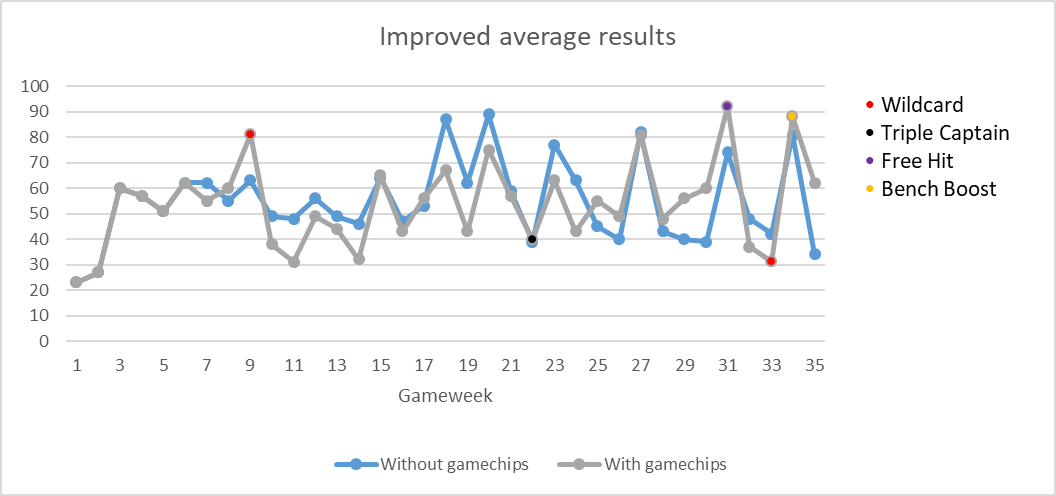
\includegraphics[scale=0.80]{fig/chapter_7/Gamechips_vs_without_colour.png}
    \caption{Comparing performance with and without gamechips}
\label{With_Without_Chips}    
\end{figure}

From figure \ref{With_Without_Chips} its observable that the two models perform identically in the first 6 gameweeks. As mentioned in section \ref{Ch.5_Game_chips} the model was allowed to use a wildcard in gameweek 9, hence this decision was first considered in gameweek 7 due to the optimization horizon of three gameweeks. Therefore, the models make different decisions from that point on. Immediately after the wildcard was played in gameweek 9, the two models tend to fluctuate greatly from one another. As 11 transfers were made using a wildcard, the two teams' starting lineup became relatively different from this point on. Unfortunately, the wildcard had a poor impact for the upcoming gameweeks, being outperformed by the other model in 10 of the following 13 gameweeks. Further, in gameweek 22, the triple captain chip was used, selecting Harry Kane as the captain. However, as Kane performed poor in those two matches, the triple captain chip had a rather weak impact on the total points gained. From this point on, the model including the gamechips tends to outperform the other model for the rest of the season. In gameweek 31, it plays the free hit gamechip due to a blank gameweek. For this particular gameweek, it greatly outperforms the other model as the free hit ensured that each player on the team was featured in that gameweek. In comparison, the model without the gamechips only had 5 players that were featured in gameweek 31. The second wildcard was played in gameweek 31, preparing for the double gameweek 34 and the blank gameweek 35. From figure \ref{With_Without_Chips} its observable that the bench boost chip was used in gameweek 34, yielding a total of 88 points. 
\newpar
With the improved average solution approach, the model obtains a total score of 1881 points when including the gamechips and 1916 points when disregarding them, yielding means of 53.743 and 54.743 points. Compared to the overall Fantasy Premier League standings, they would finish among the top 12th and 8th percentile respectively. As the model disregarding the gamechips outperforms the other with 35 points, its results will be further discussed. Figure \ref{Results_average} provides an overview of the model's weekly performance when forecasting the results using the average method. In addition, it compares its weekly performance to its mean points over the 35 gameweeks. 
\begin{figure}[H]
    \centering
    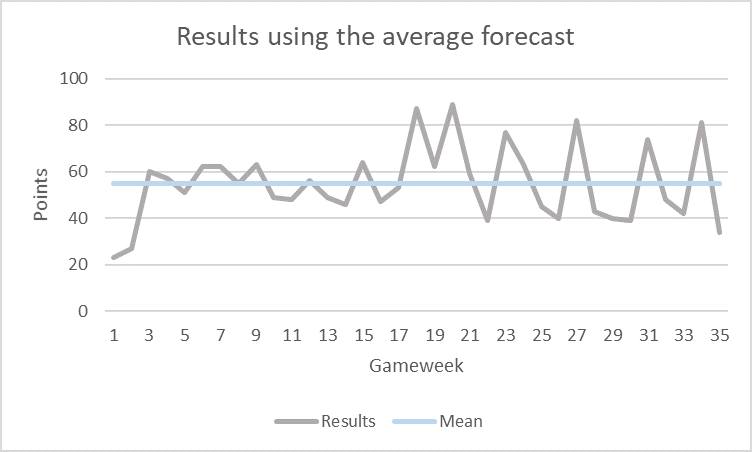
\includegraphics[scale=0.80]{fig/chapter_7/Results_average.png}
    \caption{Results using improved average as forecast}
\label{Results_average}    
\end{figure}
For the first two gameweeks the model performs rather poor compared to its mean, scoring 23 and 27 points in gameweek 1 and gameweek 2 respectively. Furthermore, its performance is stabilized around the mean score from gameweek 3 to gameweek 17. In the second part of the season, the results tend to fluctuate with greater variance around its mean. 
\begin{figure}[H]
    \centering
    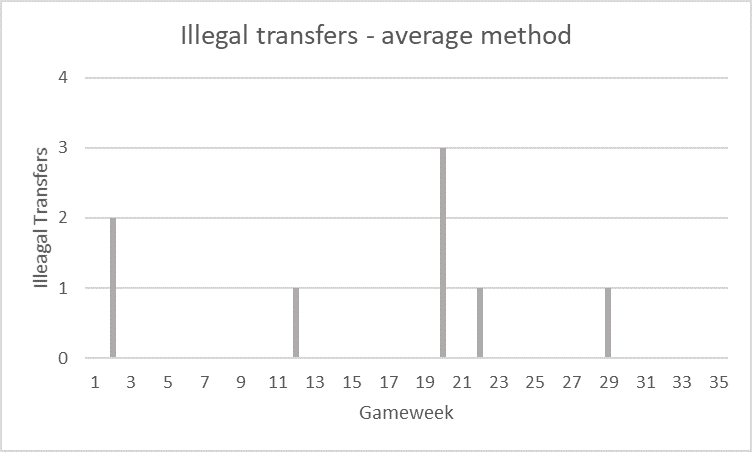
\includegraphics[scale=0.80]{fig/chapter_7/Transfers_average.png}
    \caption{Penalized transfers made using the improved average approach}
\label{Transfers_average}    
\end{figure}
Figure \ref{Transfers_average} gives information of how many penalized transfers the model performs in every gameweek. From the figure one can see that the model performed two illegal transfers ahead of gameweek 2, deducting 8 points for this gameweek. These transfers were made as Gary Cahill and Cesc Fabregas, who was selected in the initial gameweek, both received a red card in their first match. In fact, Gary Cahill was selected as captain in gameweek 1, which resulted in a score of -6 points for Gary Cahill. Hence, the sending offs and the transfers afterwards can to some degree explain the poor results in the first two gameweeks. Furthermore, its observable that the model only performs 8 penalized transfers over the entire season, which is reasonable compared to human managers. However, the model tends to finish below its mean for all the gameweeks where it performs illegal transfers. At first glance, this might seem odd. However, as the optimization horizon is set to 3 gameweeks, the model's objective is to maximize the points over the next three gameweeks, not only for the next gameweek. 

\begin{figure}[H]
    \centering
    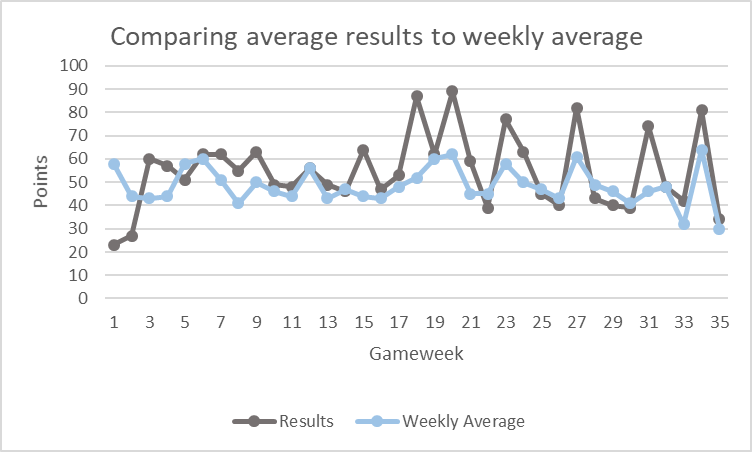
\includegraphics[scale=0.80]{fig/chapter_7/Comparison_average.png}
    \caption{Comparing improved average results to weekly average}
\label{Comparison_average}    
\end{figure} 
According to figure \ref{Comparison_average} it is obvious that the results from this solution approach greatly outperform the weekly average managers. Actually, it outperforms the weekly average in 23 of the 35 gameweeks, while it ties the weekly average in two of the gameweeks. The model is heavily beaten by the weekly average in the first two gameweeks, which is not surprising due to its poor performance in these gameweeks. Further, it seems to stabilize around the weekly average until gameweek 17. As stated when discussing the performance compared to its mean, the model tends to perform best in the second half of the season. This is confirmed by figure \ref{Comparison_average}, as the model heavily outperforms the weekly average from gameweek 18 to gameweek 35, with a total of 165 points. 

\subsubsection{Comparison to the solution approach suggested by \cite{Bonomo}}
In the following, we present a comparison between our improved average approach without gamechips to the one suggested by \cite{Bonomo}.
\begin{figure}[H]
    \centering
    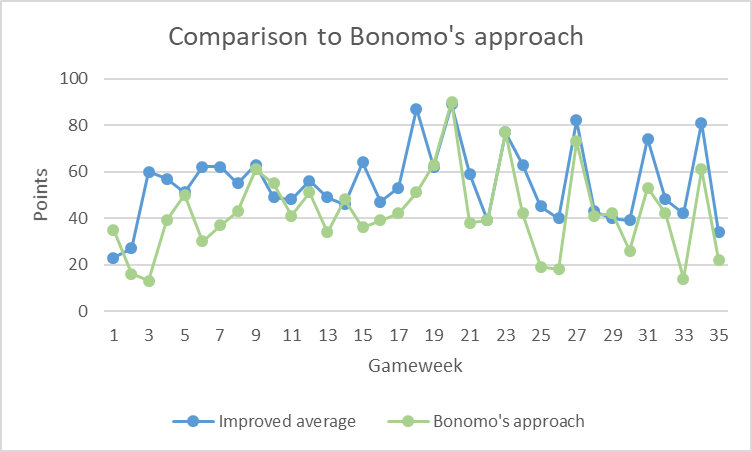
\includegraphics[scale=0.80]{fig/chapter_7/Points_vs_bonomo.png}
    \caption{Points achieved with the different approaches}
\label{Points_Bonomo}    
\end{figure}
Figure \ref{Points_Bonomo} gives a weekly comparison of the two solution approaches suggested. Clearly, the improved average outperforms the approach suggested by \cite{Bonomo} over the entire season. In fact, the improved average receives a higher score in 28 of the 35 gameweeks considered, only being defeated in 5 of the remaining gameweeks.
\begin{figure}[H]
    \centering
    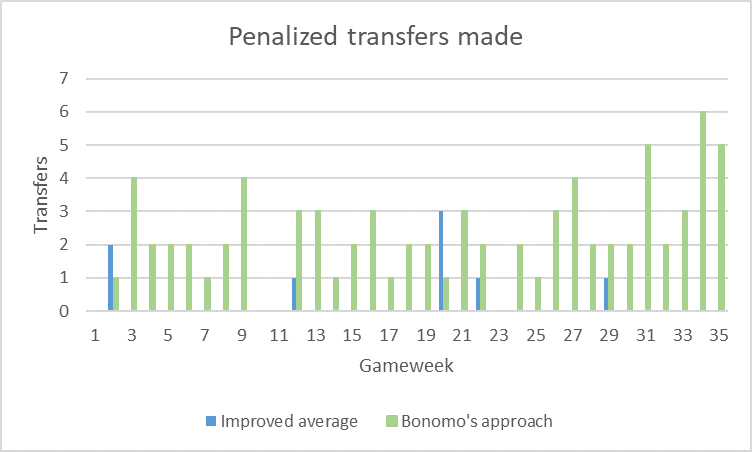
\includegraphics[scale=0.80]{fig/chapter_7/Transfers_vs_Bonomo.png}
    \caption{Penalized transfers made with the different approaches}
\label{Transfers_Bonomo}    
\end{figure}
One of the main reasons for the big difference in points scoring, is due to penalized transfers made as observed in figure \ref{Transfers_Bonomo}. As the approach suggested by \cite{Bonomo} is forced to set the illegal transfer penalty equal to 4 points, it automatically performs more penalized transfers than the improved average. In addition, \cite{Bonomo} has fixed values for the forecasting horizon and the optimization horizon, taking values of 3 gameweeks and 1 gameweek respectively. As the improved average clearly outperforms the other solution approach, the latter will not be further discussed in this chapter.

\subsubsection{Analysis of the results}
As mentioned in the previous section, the improved average method as well as the approach suggested by \citep{Bonomo}, perform poorly in the first two gameweeks. This poor performance requires further discussion. Firstly, one can argue that the models perform poorly as they both pick Gary Cahill and Cesc Fabregas, who both received a red card in the first gameweek. With Cahill listed as captain, they deduct a total of -7 points. Further, is a result of poor forecast for the first three rounds. Hence, players that performed well in the previous season had a rather weak start of this season. In fact, from the previous season's dream team, i.e. the 11 players that collected most points, only one of them had a score above two points in the first gameweek. In addition, one can argue that the poor performance in the first gameweeks is due to we exclude players that were transferred to Premier League ahead of the season. Hence, players like Mohamed Salah, Alvaro Morata and Alexandre Lacazette were not included in the first gameweek. 
\newpar
From figure \ref{Comparison_average} we see that the results tend to stabilize around the weekly average from gameweek 3 until gameweek 18. The reason why is that the forecast now includes the realized points from gameweek 1 and 2, hence it is able to capture which players who had a good start to the season. In addition, the transferred players from outside Premier League, including the newly promoted teams, are now included to the model. One can argue that the forecast improves during the season, being able to capture which players that are performing well at different points of time. 
\newpar
In the second part of the season, the improved average method greatly outperforms the weekly average managers. Firstly, it is due to an improved forecast, which performs better over time. Secondly, it can be due to human players quitting during the season. If a human manager has performed poorly in the first half of the season, it is not unreasonable to assume that he quits playing to some degree. Hence, as a result of managers loosing interest to the game during the second half of the season, it is expected that the weekly average is affected in terms of decreased points.
\newpar
Readers may be surprised by the fact that the improved average performs better when disregarding the gamechips than when including them. Intuitively, one would think that the gamechips should have a positive effect, thus increasing the total points. As dicussed in section \ref{Average_results}, the improved average models perform equally until the wildcard is considered first in gameweek 7. By transferring 11 players in gameweek 9 using a wildcard, the starting line-up of the improved average including gamechips differs greatly from that disregarding them. Intuitively, based on the forecasts the one including the gamechips should outperform the other one for the following gameweek, as it allows for maximizing the expected score over the next three gameweeks without any penalized transfers. However, as observed in figure \ref{Comparison_average} this is not the case. This is due to the fact that the forecasts were not good enough to predict which players that were going to perform best for the next gameweeks. After all, football is a game of uncertainty and one can never know exactly how a player will perform in the future. Therefore, one can actually argue that the model was unlucky when playing the wildcard, as the new players did not outperform the old ones as expected. 
\newpar
The reason why the two models differ greatly for the rest of the season, is in fact due to the wildcard played in gameweek 9. Further, from figure \ref{Comparison_average} its observable that the triple captain had a positive impact to some degree. Also, it is observable that the model including the gamechips heavily outperform the other one in gameweek 29 to 31. This can be due to the free hit played in gameweek 31. While the model disregarding the gamechips has to prepare for the blank gameweek 31 and thus make transfers accordingly, the one including the wildcards knows that it has the possibility to play the free hit in that particular gameweek. Hence, one can argue that the free hit chip had a positive impact in gameweek 29 to 31 for the model including the gamechips. 
\newpar
Finally, we see that the wildcard and the bench boost in gameweek 33 and 34 respectively had a positive effect for the total score. In addition, the wildcard gives a positive impact for gameweek 35, as it prepare for this one as well when deciding which transfers to make in gameweek 33. 
\newpar
In order to conclude the discussion above, one can argue that the first wildcard had a severe negative impact in the first half of the season. However, as mentioned above there is a high uncertainty related to football, one can never ensure that your prediction is correct. 
As for the triple captain and the bench boost chips, they should not have a negative effect if the starting line-up is held constant over the season. Well, one can argue that the captain can receive a red card or that the players on the bench earn negative points, but the probability of this negligible. 

\begin{comment}

Possible metrics: 

Results of total sum, average, predicted points pr round opp mot actual points pr round, computational time, st.dev highest round, lowest round, number of illegal transfers, when gamechips are used, "case-study"



- Summarizing conclusion based on the variance/standard deviation of each method.
- Say something about the computational time for each method. 


\begin{table}[H]
\centering
\caption{Results of total sum, average, total sum best player. Model without variance.}
\begin{tabular}{llllll}
& Our Method & Our Method w/var  & Average Players & Best Player & Exact\\
Total sum  & NA  & NA & NA & NA & NA \\
\end{tabular}
\end{table}



\textit{Case-study of round w/chip to show that the model makes sense}
\end{comment}


 \begin{comment}
 tabell 1: total sum points after gameweek 35, total mean for each round, ranking. 

forklare minst og høyeste antall illegal transfers og referere til appendiks. 

graf 1: poeng hver runde, average for hver runde i selve spillet, når gamechippene brukes,
 \end{comment}



\newpage
\subsection{Regression Model}
With the solution approach using a linear regression, our model obtain an average score of 49.22 points in the first 35 gameweeks. With this average, the model perform among the top 36\% on the FPL overall ranking. Figure \ref{Regression_results} provide the score for each gameweek compared to the mean of 49.22 points. 

\begin{figure}[H]
    \centering
    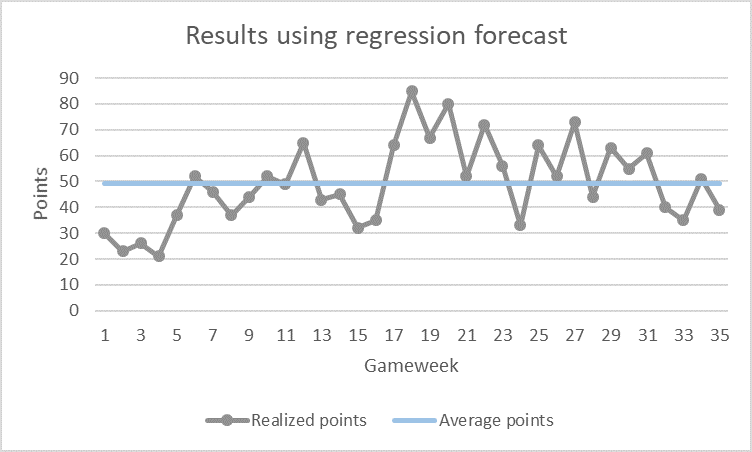
\includegraphics[scale=0.75]{fig/chapter_7/Regression_results.png}
    \caption{Results using regression as forecast}
\label{Regression_results}    
\end{figure}

From the figure it is noteworthy that the model performs poorly in the first 5 gameweeks. Further, it seems to stabilize among its mean managers from gameweek 6 to gameweek 16. An interesting observation is that the model largely outperforms its mean in the second half of the season. The poor performance in the first gameweeks can to some degree be explained by figure \ref{Transfers_regression} which provides an overview over illegal transfers made ahead of each gameweek.

\begin{figure}[H]
    \centering
    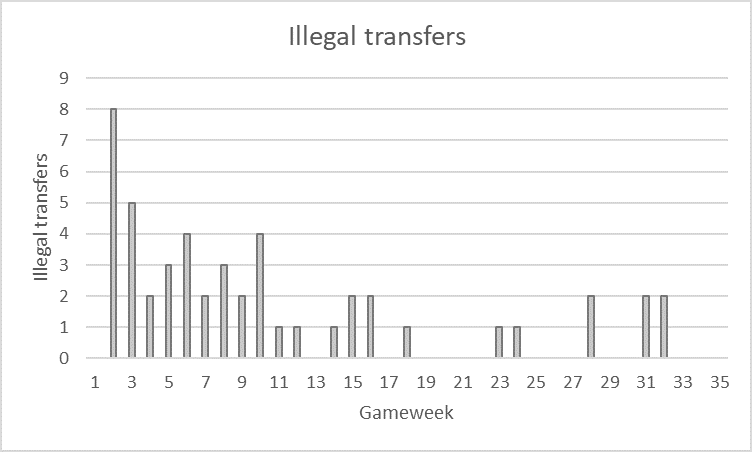
\includegraphics[scale=0.75]{fig/chapter_7/Transfers_regression.png}
    \caption{Penalized transfers made using the regression approach}
\label{Transfers_regression}    
\end{figure}

As easily observed, the model frequently executes illegal transfers in the first 10 gameweeks. For instance, ahead of gameweek 2 it allows for 8 illegal transfers, deducting a total of 32 points from the overall score. The transfers are mainly due to players that over- and under-performed compared to last season's performance. In addition, the model does not consider players that were transferred from outside of the Premier League. Hence, a player like Mohamed Salah who is by far the top points scorer was not considered in the first gameweek. As the number of illegal transfers decreases in the second half of the season, the model tends to perform better. Thus, one can argue that the model makes too many illegal transfers early in the season and that this influence the overall points to a large degree. 
\newpar
A comparison of the results from the regression approach to the human average performance in each gameweek is made in figure \ref{Regression_vs_average}.

\begin{figure}[H]
    \centering
    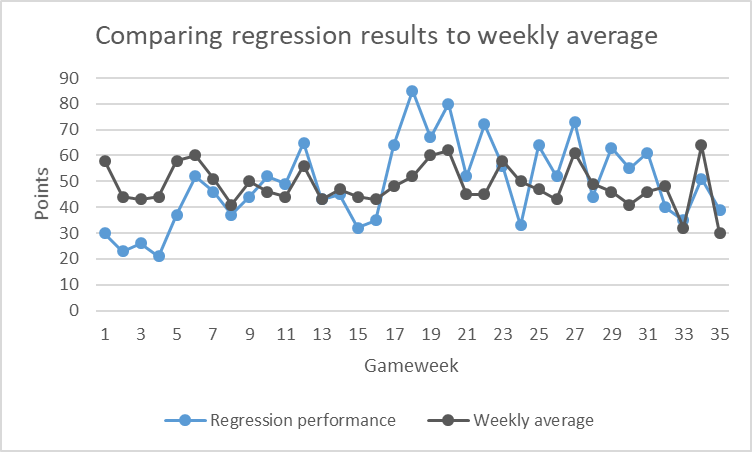
\includegraphics[scale=0.75]{fig/chapter_7/Weekly_average_regression.png}
    \caption{Comparing regression approach to weekly average}
\label{Regression_vs_average}    
\end{figure}

As expected from figure \ref{Regression_results}, the model is outperformed by the average human managers in the first gameweeks. This is as mentioned due to the frequently usage of illegal transfers. In the first 9 gameweeks, the average managers outperform the model by a total of 133 points. However, over the entire season (35 gameweeks in this case) the model outperforms the average managers by a total of 24 points, which is considered to be a good result considering the poor start of the season. As we reach gameweek 17, the model outperforms the average managers in 14 of the remaining 19 gameweeks. Firstly, this is due to the model adopting which players that have performed best over the season. Secondly, the decrease of illegal transfers is an important factor. However, it has to be mentioned that as time goes by some human managers tend to quit playing FPL as a result of a bad start. Hence, it is likely that the average would have been slightly higher if some managers did not quit during the season. 

\subsection{Odds}


\subsection{Summary}
Here we present a table that summarizes the results from the three different approaches. 




\begin{comment}
\section{Recommendations for human FPL managers}
- hvilke anbefalinger kan man gi til fpl managere? 
     * hvilke formasjon går igjen i løsningene. lønner det seg med forsvarsspillere eller angrepsspillere?  
    * er budsjettet alltid oppfylt? og hvordan utvikler verdien til laget seg over sesongen? 
    
    - Tabell over Formasjon i optimal solution. 



\begin{table}[H]
\centering
\caption{Results of total sum, average, total sum best player. Model without variance.}
\begin{tabular}{llllllll}
& Average Argentina & Average Improved & Odds & Regression  & Average Players & Best Player & Exact\\
Total sum  & NA  & NA & NA & NA & NA & NA & NA \\
\end{tabular}
\end{table}
\end{comment}

\begin{comment}
Good discussion points: 
\begin{enumerate}
    \item hvis man legger restriksjon på formasjon. Hvilke formasjon gir mest poeng?
    \item når bruker man de forskjellige chippene, og hvor effektive er de?  
\end{enumerate}
\end{comment}


\section{Case study: How variance influence the solution.}

In this section the variance constraints presented in Section \ref{Ch.5_Variance_tradeoff} are added to the mathematical model, and the results 



\begin{enumerate}
    \item plot with the objective value and threshold. the objective value is the accumulated objective value of the model run over all gameweeks. 
    \item explanation of the graph and discussion 
    \item plot with the realized points and threshold. 
    \item explanation of the graph and discussion. 
    \item 
\end{enumerate}
Remember: similar to efficient frontier with expected points